%%%% 
% This is a template for project reports in the subject DAT620 at the
% Department of Electrical Engineering and Computer Science,
% University of Stavanger.
% 
% The template is based on the ACM conference template 
% it was edited by Leander Jehl and Hein Meling

\documentclass[sigconf]{acmart}
\usepackage{hyperref}

%DON'T CHANGE THIS FILE
%This file sets several properties for the ACM template.
%It is not necessary to change this file.


% Copyright
\setcopyright{none}

% DOI
\acmDOI{}

% ISBN
\acmISBN{}

%Conference
\acmConference
\acmBooktitle
\copyrightyear{}

\newcommand{\supervisors}[1]{\thanks{Supervised by #1}}


%In the preamble file you can include packages and define macros.
\usepackage{xspace}

%Here we define a marco: The \xspace ensures correct spacing, i.e. insert space before next word, but not before period or comma.
\newcommand{\paxos}{\textsc{Paxos}\xspace}

%These packages are needed for the plot in Figure 1. 
\usepackage{tikz}
\usepackage{pgfplots}
\pgfplotsset{compat=newest}



\begin{document}
%TODO: Replace the title with your project title.
\title{HackerSearch: an Information Retrieval system}
%you may use a subtitle
\subtitle{Milestone 1}

%TODO replace author names with your name and email below:
\author{Ana Barros}
\affiliation{FEUP}
\email{up201806593@edu.fe.up.pt}

\author{João Costa}
\affiliation{FEUP}
\email{up201806560@edu.fe.up.pt}

\author{João Martins}
\affiliation{FEUP}
\email{up201806436@edu.fe.up.pt}

%TODO: add the name of one or more supervisors
\supervisors{Sara Fernandes and Sérgio Nunes}

\begin{abstract}
    In this project, textual data, corresponding to the year 2018, was
    collected from the ``HackerNews'' link aggregator and corresponding
    linked URLs. After refinement and analysis, this data will be used
    to develop an Information Retrieval system.
\end{abstract}

%TODO: Replace with some keywords, relevant for your project
\keywords{datasets, information retrieval, search engine, HackerNews,
Y Combinator, HackerSearch, data analysis}

\maketitle

%Each section can be placed in a separate file and included by the input command.

\section{Introduction}
\label{sec:introduction}
``HackerNews'' is a link aggregator website, mainly used to share news
and products. It focuses on tech-related topics, such as computer science,
and entrepreneurship. ``HackerNews'' is backed by ``Y Combinator''
foundation, which funds early startups biannually.\\
The community in this website usually interacts by sharing links to
articles (blogs, news websites, and product landing pages) and then,
voting and commenting on them. What sets this community apart is the
vast technical knowledge shown in most comments, giving them a high
readability value which sometimes surpasses the value of the post
discussed.

This article aims to describe the first milestone of the development
of ``HackerSearch''. This platform will serve as an intuitive and
powerful search engine for ``HackerNews'' posts/content.\\
This report is divided into 2 main sections. Each of these sections
describes different tasks completed in order to achieve the final
goal for this \textbf{milestone: data preparation}. The first section,
\hyperref[sec:collection]{Data Collection}, describes the process
of retrieving the data. The second section, 
\hyperref[sec:processing]{Data Processing}, describes the filtering 
and preparation of the gathered data.
The final section, \hyperref[sec:analysis]{Data Analysis}, lists 
the process of exploring the data with statistics, 
characterizing the final datasets and their properties, the conceptual 
model as well as the follow-up information needs in the data domain. 

\section{Data Collection}
\label{sec:collection}
``HackerNews'' provides an \textit{official public API} \cite{API}
to fetch website's data. This data is output in \textbf{JSON format},
and the \textbf{curl} command line utility is used to fetch it.

\subsection{Posts/Stories}
\label{sec:collection_posts}
There are three types of posts in ``HackerNews'': \textbf{story},
\textbf{job}, and \textbf{poll}. It was decided that our dataset
would only contain stories, as those comprise around $99.99\%$ of
posts on the website. From now on, all references to post/story
are interchangeable.

The API \cite{API} does not provide a way to perform bulk downloads. In order
to streamline the process of fetching data, a starting dataset
\cite{githubDataset} was used. This dataset contained the raw data
of stories collected using the API \cite{API}. It is fetched by cloning the
GitHub repository using the git command-line utility. The data
comes divided into several JSON files containing a single list
with multiple objects representing stories. This was done to
bypass GitHub's limit on file size. Upon downloading, these
lists are joined into a single one using the \textbf{jq} \cite{jq}
command-line utility, so the stories can be filtered more easily
and stored in the \textbf{stories.json} file.\\
Given the large volume of data available, it was decided
to only deal with information related to stories posted in
2018. This is equivalent to around 50000 stories.

\subsection{Comments}
The dataset mentioned above only contains data about stories. To
complement this, the API \cite{API} was used to download the data of the
top two comments of each story. This translates to around
100000 comments.\\
To download this data, curl with persistent connections was used,
thus reducing the time expended establishing connections with
the API \cite{API}, and multiple sub-processes, to parallelize work. In
order to easily parallelize the work and make use of persistent
connections in curl, it was necessary to use a file containing URLs
as input. This file was built using \textbf{jq} \cite{jq} (to select the
IDs of the top comments) and \textbf{awk} (to build the URLs using
the IDs that were being piped). Afterwards, it was split info
multiple files (one for each sub-process) using GNU's split,
so each sub-process could take care of their part of the URLs.

\textbf{Jq} \cite{jq} was used to concatenate all the downloaded comment
data into a single JSON list stored in the \textbf{comments.json}
file.

\subsection{URL content}
As stories without a link are frowned upon on ``HackerNews'', most
stories ($90\%$) do not have textual content (apart from the title).
Instead, users are incentivized to share URLs to the content they
want to discuss/share. This limits the searchability of stories.

To work around this, a small program was developed using
Mozilla's Readability tool \cite{readability} (part of the Firefox
browser) to fetch the main content of the URLs linked by the stories
in text form. This allows us to perform general web scraping
in many websites with different layouts/content, which wouldn't
be feasible with a specialized 'web spider'.\\
This code uses \textbf{node-fetch} \cite{node-fetch} to fetch the
target website's data and \textbf{jsdom} \cite{jsdom} to feed this
data to the readability tool \cite{readability}.

\textbf{Jq} \cite{jq} is used to select the stories containing
a URL, and GNU's split is used to divide the information of these
stories into multiple files (each used by a respective sub-process).
The website's extracted textual content is stored in a JSON
object alongside its post ID. Each sub-process stores the
content it is responsible for in a file. The JSON objects in
these files are subsequently concatenated into a single JSON
list using \textbf{jq} \cite{jq} and stored into the
\textbf{html\_content.json} file.

\section{Data Processing}
\label{sec:processing}

\begin{figure*}[htb!]
   \centering
   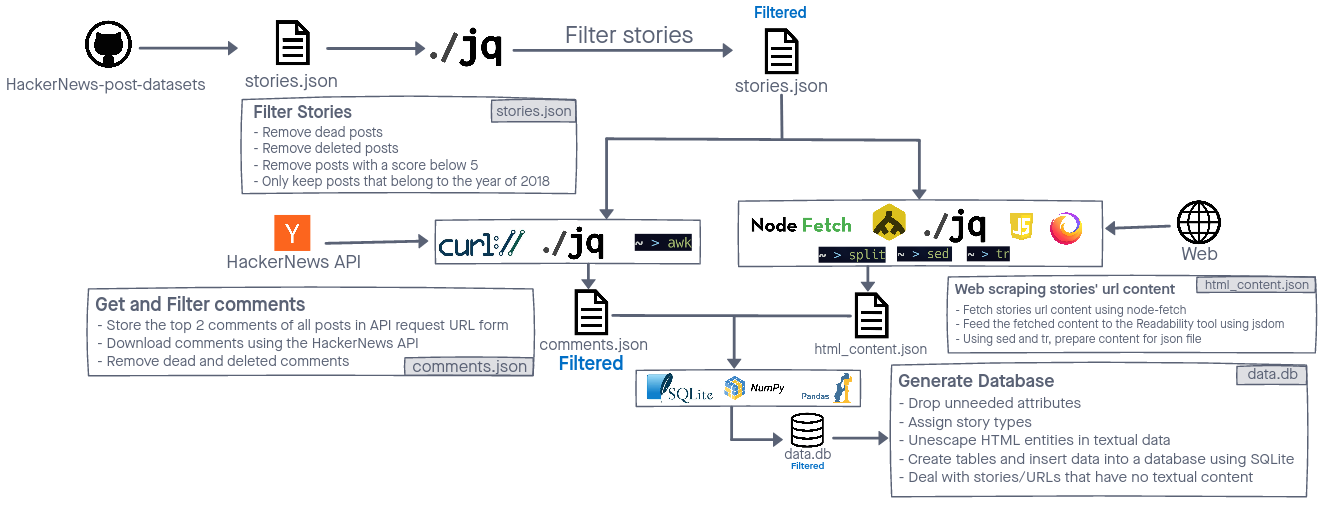
\includegraphics[width=\linewidth]{fig/dataflow_diagram.png}
    \caption{Dataflow Diagram}
    \label{fig:dataflow_diagram}
\end{figure*}

While being collected and before being analyzed, the data is passed
through a pipeline where it was transformed and filtered.

\subsection{Initial Processing}
The processing and filtering processes described in this
subsection were applied during the data collection process.

In order to reduce the number of stories (while increasing their
relevance), they were filtered out based on the following criteria:
\begin{itemize}
    \item Stories deleted by their owner.
    \item Dead stories (flagged by the users): If a story is reported
        by enough users, it is deleted.
    \item Stories that 'failed': A story 'fails' when it scores
        lower than 5 points, thus not being able to reach the front
        page of the website. Every story starts with 1 point and gains
        1 extra point for each vote it receives.
\end{itemize}
These filtering steps were all performed by a single \textbf{jq}
\cite{jq} script that encompasses all conditions mentioned above.

Comments suffered a similar filtering process (using \textbf{jq} \cite{jq}):
dead and deleted comments were filtered out.
It should be noted that some less popular stories have less than
2 comments in the final dataset, because users might not have
engaged enough in their discussion or all their comments were filtered
out for the reasons above.

The content of the URLs of the stories isn't always useful as textual
data: some URLs link to binary data (images, PDF files, videos, etc...)
and others might lead to web pages that our tool isn't able to extract
information from (e.g.: YouTube's website). In these cases where the URL
doesn't lead to any useful information and the story does not have
textual content, it was decided to 'drop' this from the dataset.\\
When the URL yields useful information (most cases), the yielded
data is compressed to remove repeated blank spaces and newlines,
and filtered to remove non-printable characters. This is done using
a series of piped \textbf{sed} and \textbf{GNU's tr} commands. These
processes are important because the website data is frequently
unstructured and large.

\subsection{Post-Processing}
\label{sec:post_processing}
After all the data was gathered, it was necessary to perform some
final cleanups and save it in a more fitting format: at this point,
the data was saved in three JSON files which needed to be unified.

The 3 JSON files containing the data were imported into python's
\textbf{pandas \cite{pandas} DataFrames} to be worked on. The steps described
below were taken using the \textbf{pandas\cite{pandas} and numpy \cite{numpy}} modules in
python3.

All the stories in the dataset had a \textbf{type} field with
the value \textbf{story}. This happened because only the posts
of that type were downloaded (as mentioned in the
\hyperref[sec:collection_posts]{Posts/Stories Data collection
subsection}. This field was replaced by a new one of the same
name that divides the stories into the dataset in four categories,
recognized by the ``HackerNews'' website, that can be filtered in
their tabs. These categories are:
\begin{itemize}
    \item \textbf{LaunchHN} - these are stories about new
        ``Y Combinator'' backed start-ups. This type of stories
        start their title with \textit{``Launch HN:''}.
    \item \textbf{AskHN} - these are questions to the website's
        community. This type of story can't have a URL, and their
        title almost always starts with \textit{``Ask HN:''}.
        Every story that doesn't have a URL falls in this category.
    \item \textbf{ShowHN} - these are stories that usually want to
        share a product landing/main page. This category is very
        similar to the \textbf{Normal} category discussed below,
        being only distinguished by their title starting with
        \textit{``Show HN:''} and thus being shown in their
        filtered page.
    \item \textbf{Normal} - this is the category where most
        stories fall under. These always have a URL and rarely
        contain a textual description. Most time these link
        to news and scientific articles, or blog posts.
\end{itemize}
The percentage distribution of each of these categories in
the final dataset will be discussed below in the
\hyperref[sec:analysis]{Data Analysis section}.

Both the story data and the comments contain a \textbf{'kids'}
field. This field is a list of the direct descendants of
the respective story/comment.\\
In the case of the stories, their data also contains a
\textbf{descendants} field that represents the number of
child comments in total (across all nesting levels).\\
It was decided that the \textbf{'kids'} field has no value
for the final dataset and, in the case of the comments,
should be used to derive a \textbf{descendants} field
before being dropped. This solution is not optimal as
it doesn't take into account the number of child
comments across all nesting levels, but only the top-level.
It was still decided to use this solution, as it was
infeasible to fetch the data of every comment (over
2.5 million) of the chosen stories in order to count
the number of child comments.

Some data acquired from the ``HackerNews'' API \cite{API},
namely the \textbf{text} fields of both the stories and the
comments, contained HTML special chars escapes. These were
'unescaped' so they could be stored cleanly.

\section{Conceptual Model}
\label{sec:conceptual_model}
After the gathering and passing through the data processing
pipeline, the final data on the \textbf{pandas' DataFrames}
was exported to a sqlite3 database (described in this section),
using the \textbf{sqlalchemy python module}.

\begin{figure}[htb!]
   \centering
   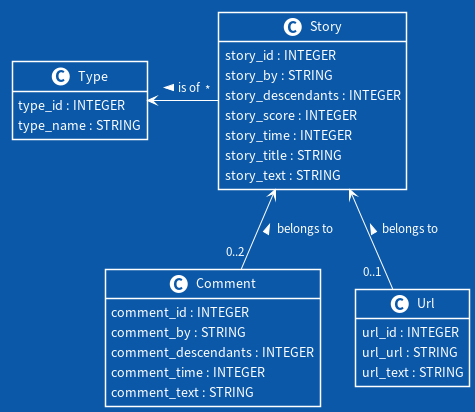
\includegraphics[scale=0.4]{fig/database.png}
    \caption{Conceptual Model}
    \label{fig:database}
\end{figure}

For the data domain, a conceptual model was created in order to 
understand the data organization. There are four tables: 
\textit{Type, Story, Comment}, and \textit{URL}. The main 
attributes of the \textit{Story} table are: 
\begin{itemize}
    \item story\_by: the username of the user who posted the story.
    \item story\_descendants: the number of comments of the story.
    \item story\_score: the score of the post (a sum of its upvotes).
    \item story\_time: the (UNIX) timestamp of when the story was posted.
    \item story\_title: the title of the story.
    \item story\_text: the textual content of the story.
    \item story\_type: the type of the story (foreign key to the \textit{Type} table). 
\end{itemize}

The \textit{Type} class exists in order to represent the type 
of story. All stories have a type. This class contains only 
two attributes:

\begin{itemize}
    \item type\_id: the integer that identifies a story type.
    \item type\_name: the name of the type. 
\end{itemize}

The \textit{Url} class represents the textual data obtained from 
URLs that are linked inside a story. Not every story needs 
to have a URL. However, a story cannot have more than one URL.
The main attributes of this table are:

\begin{itemize}
    \item url\_url: the URL of the resource.
    \item url\_text: the filtered textual contents of the 
    web resource the URL links to. These contents were obtained 
    as described in the 
    \hyperref[sec:collection]{Data Collection} section.
\end{itemize}

Finally, the \textit{Comment} table is used to represent 
a comment of a story. Each comment only belongs to one story.
Each story might have one, two, or no comments. These are its
main attributes: 

\begin{itemize}
    \item comment\_by: the user who posted the comment.
    \item comment\_descendants: the number of replies of a comment
    (as described in the \hyperref[sec:post_processing]{Post Processing subsection}.
    \item comment\_time: the (UNIX) timestamp of when comment was
    posted.
    \item comment\_text: the content of the parent story.
\end{itemize}

\section{Data Characterization/Analysis}
\label{sec:analysis}
This section describes the data characterization using graphics,
plots, and textual descriptions.

\begin{figure}[htb!]
   \centering
   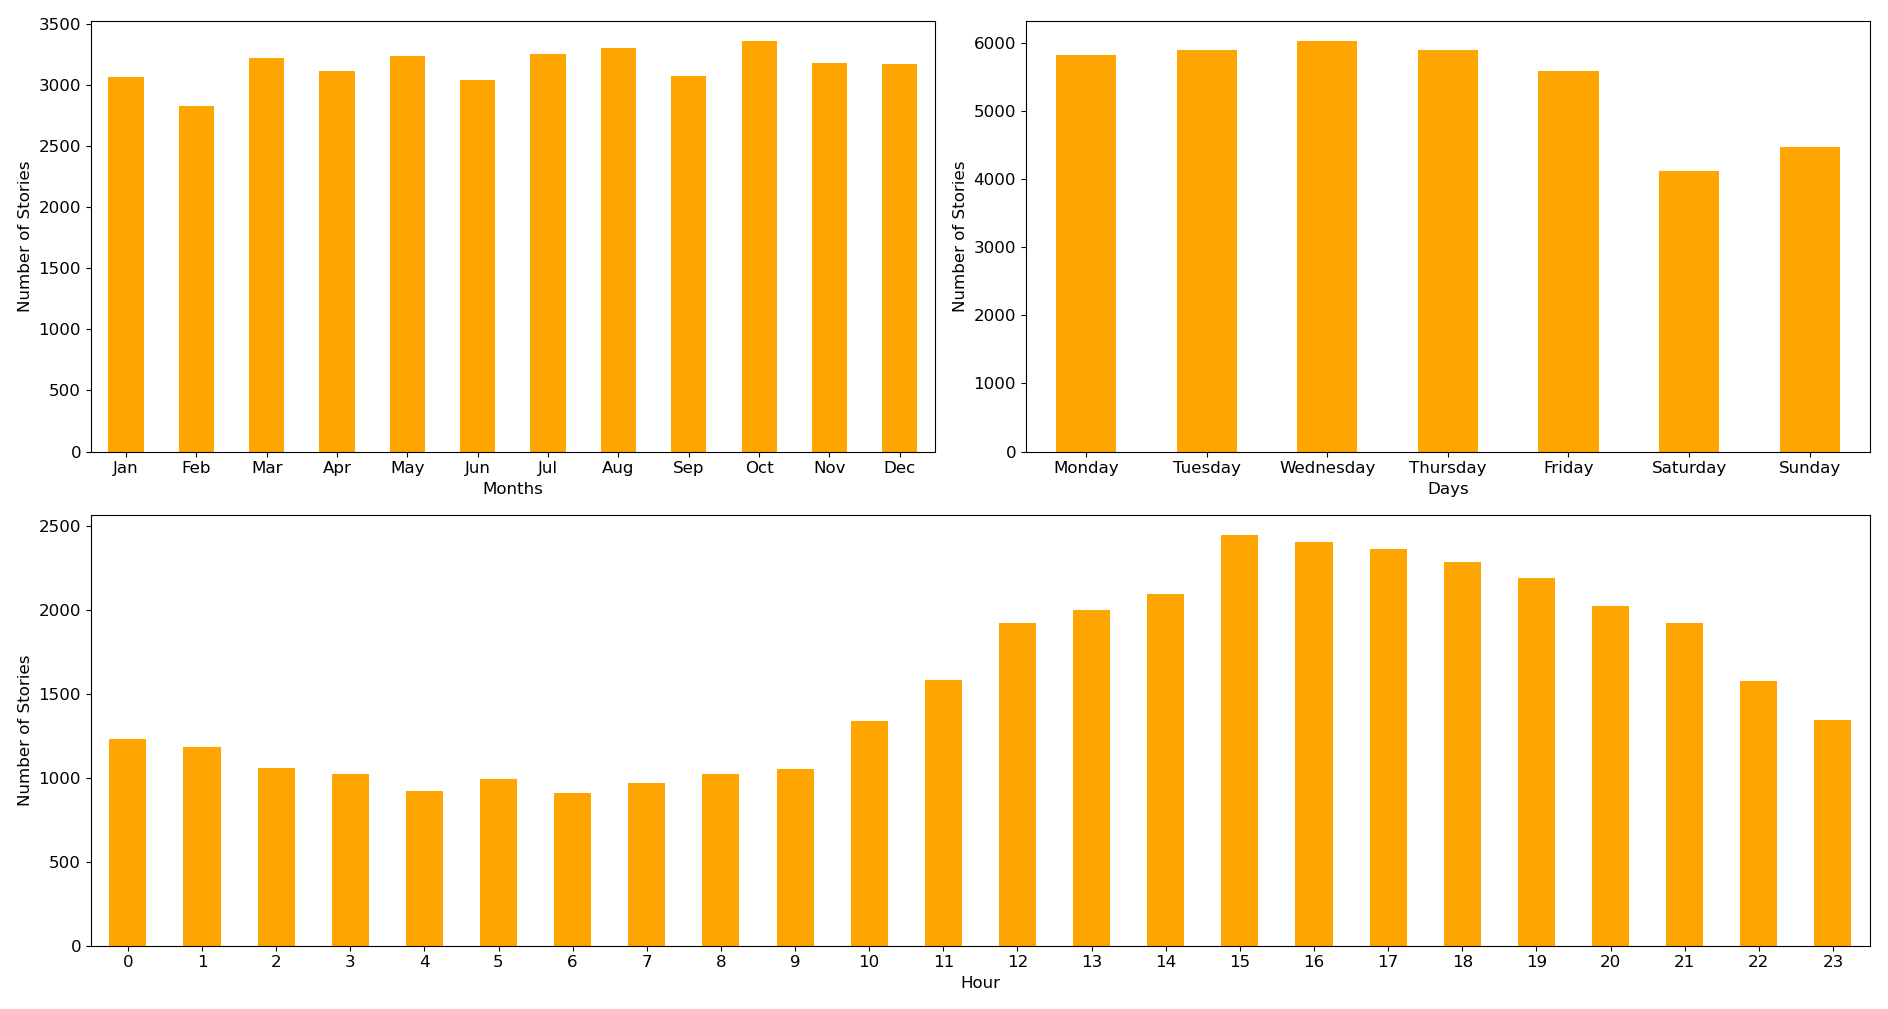
\includegraphics[width=\linewidth]{fig/stories_per_time.png}
    \caption{Number of stories per time}
    \label{fig:stories_per_time}
\end{figure}

By analyzing the dataset, it can be concluded that there is higher
frequency of story posts during the afternoon. Throughout the week,
posts are more frequent during the weekdays as in contrast with
the weekend. Finally, there is not a particular time of the year
when the number of stories posted differentiates from the rest.

The distribution of posts based on type is unbalanced. As described
previously, there are four categories of stories: ``Normal'', ``AskHN'',
``ShowHN'', and ``LaunchHN''. The reality is that $85,5\%$ of all posts
(which translates to almost 33000 posts) are classified as ``Normal''
posts while there are less than 100 posts classified as ``LaunchHN''.
This is expected considering that most posts on ``HackerNews'' intend
on sharing a news article or blog post (most common category) and
``LaunchHN'' posts are a special category for new Y Combinator startups
(less common category). The other two categories fall somewhere in between.

\begin{figure}[htb!]
   \centering
   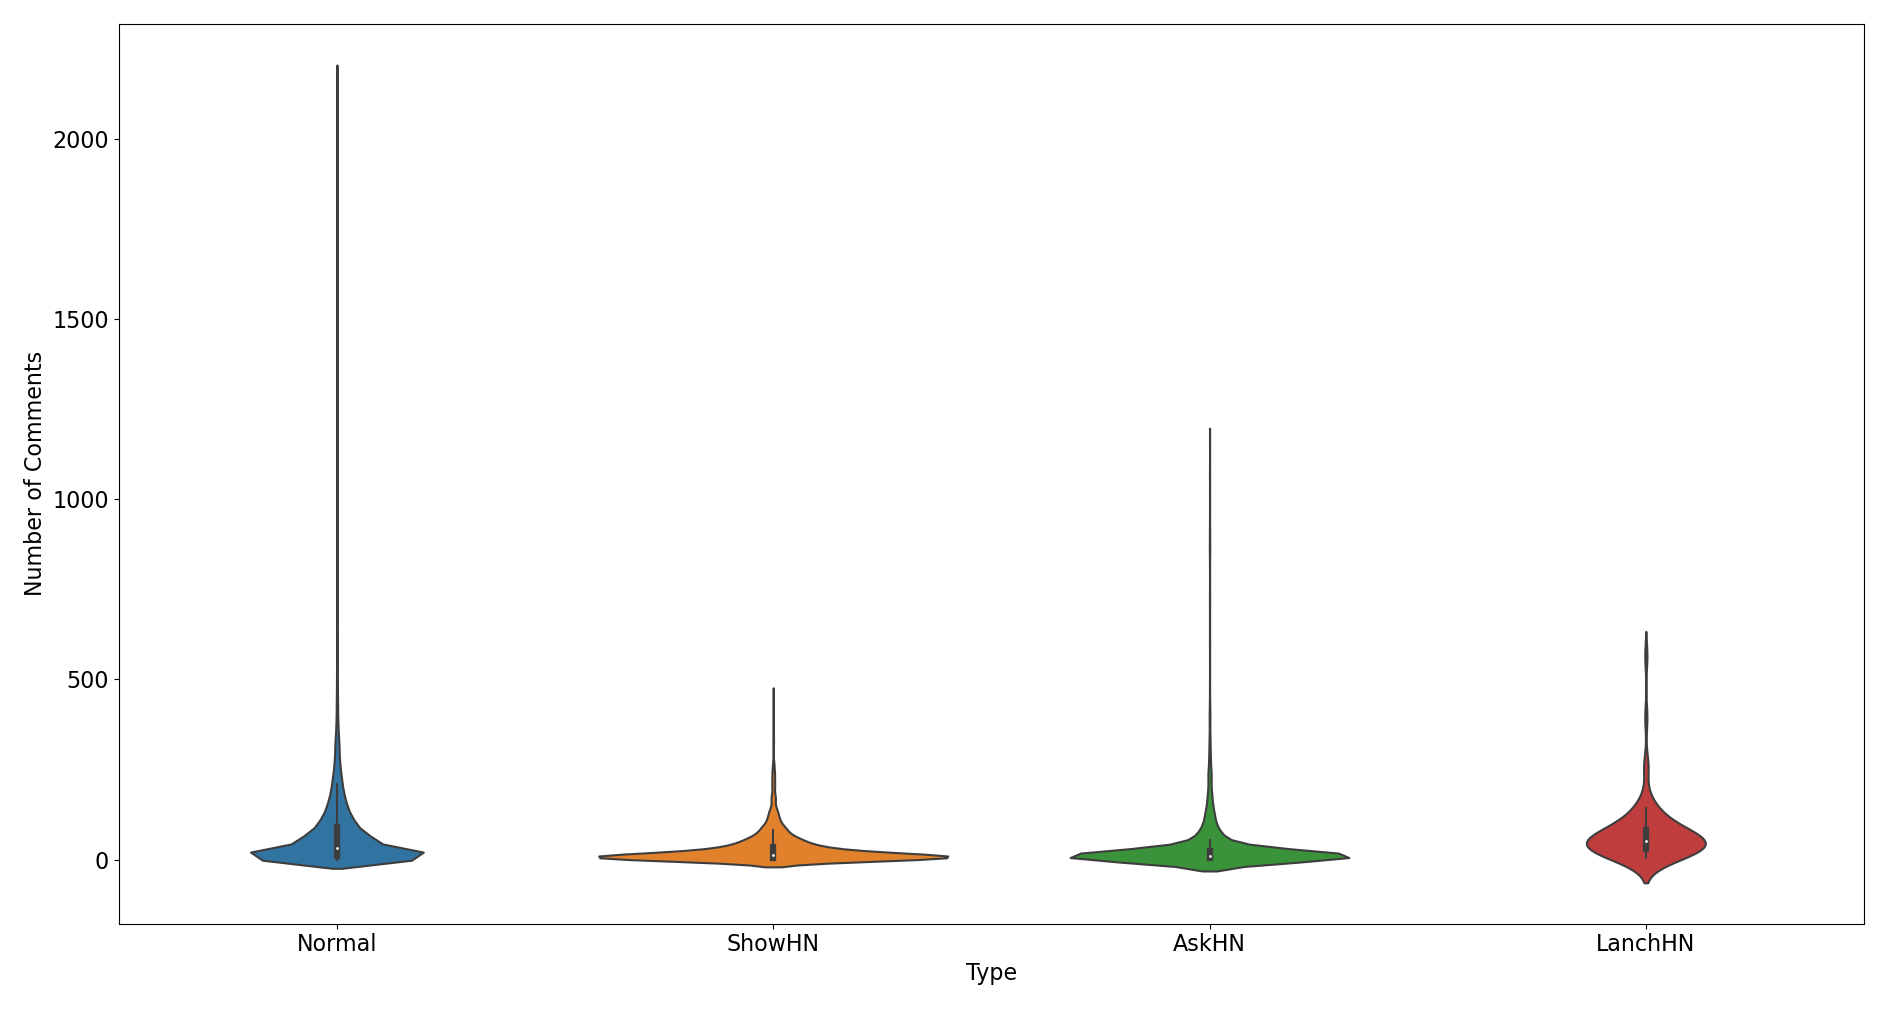
\includegraphics[width=\linewidth]{fig/descendants_per_type.png}
    \caption{Number of comments per type}
    \label{fig:descendants_per_type}
\end{figure}

`Normal'' stories have a higher ceiling for number of comments (followed
by ``AskHN''), but the median number of comments is roughly the same for
all story types. This is surprising considering that stories that do not
contain a URL (the case of ``AskHN'') are penalized in terms of exposition,
requiring more engagement from users in order to reach the front page
(succeeding).

\begin{figure}[htb!]
   \centering
   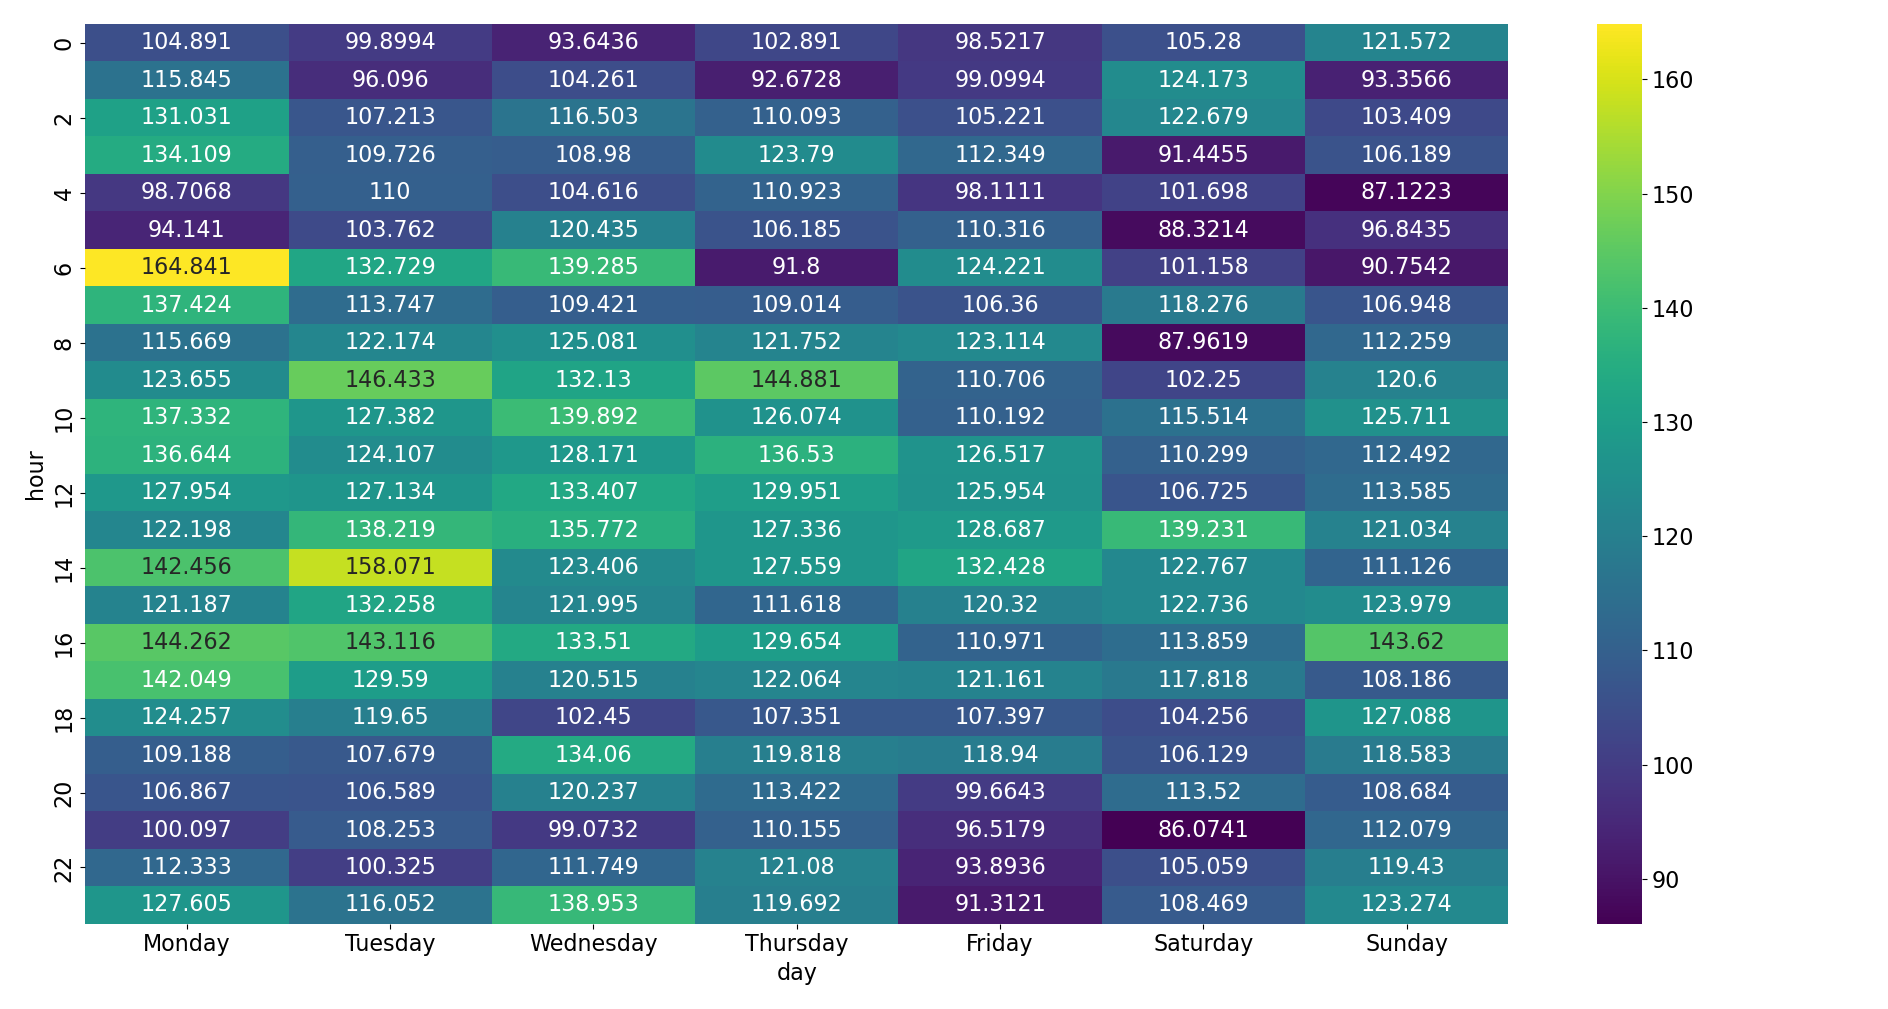
\includegraphics[width=\linewidth]{fig/heatmap_score_per_dayandhour.png}
    \caption{Average score in reference to time and day of the week}
    \label{fig:heatmap_score_per_dayandhour}
\end{figure}

By analyzing the heatmap that relates the score of a story with the time
and day of the week of when the story was posted, it can be concluded that
stories posted at the beginning of the week (Monday, Tuesday, Wednesday)
and in the middle of the day (10AM-4PM), achieve higher scores. The average
higher scores are achieved by stories posted between 6AM and 2PM on a
Monday and from 9AM to 6PM on a Tuesday. Most of the high discrepancy between
the cells with the highest score values and its neighboring cells can be
explained by the fact that most outliers occur within these timeframes.
For example, one of the highest rated stories (2776 up-votes) was posted
on Wednesday at 11PM, which has an average score of 138, while its
neighboring cells have a score of 111 and 100.

\begin{figure}[htb!]
   \centering
   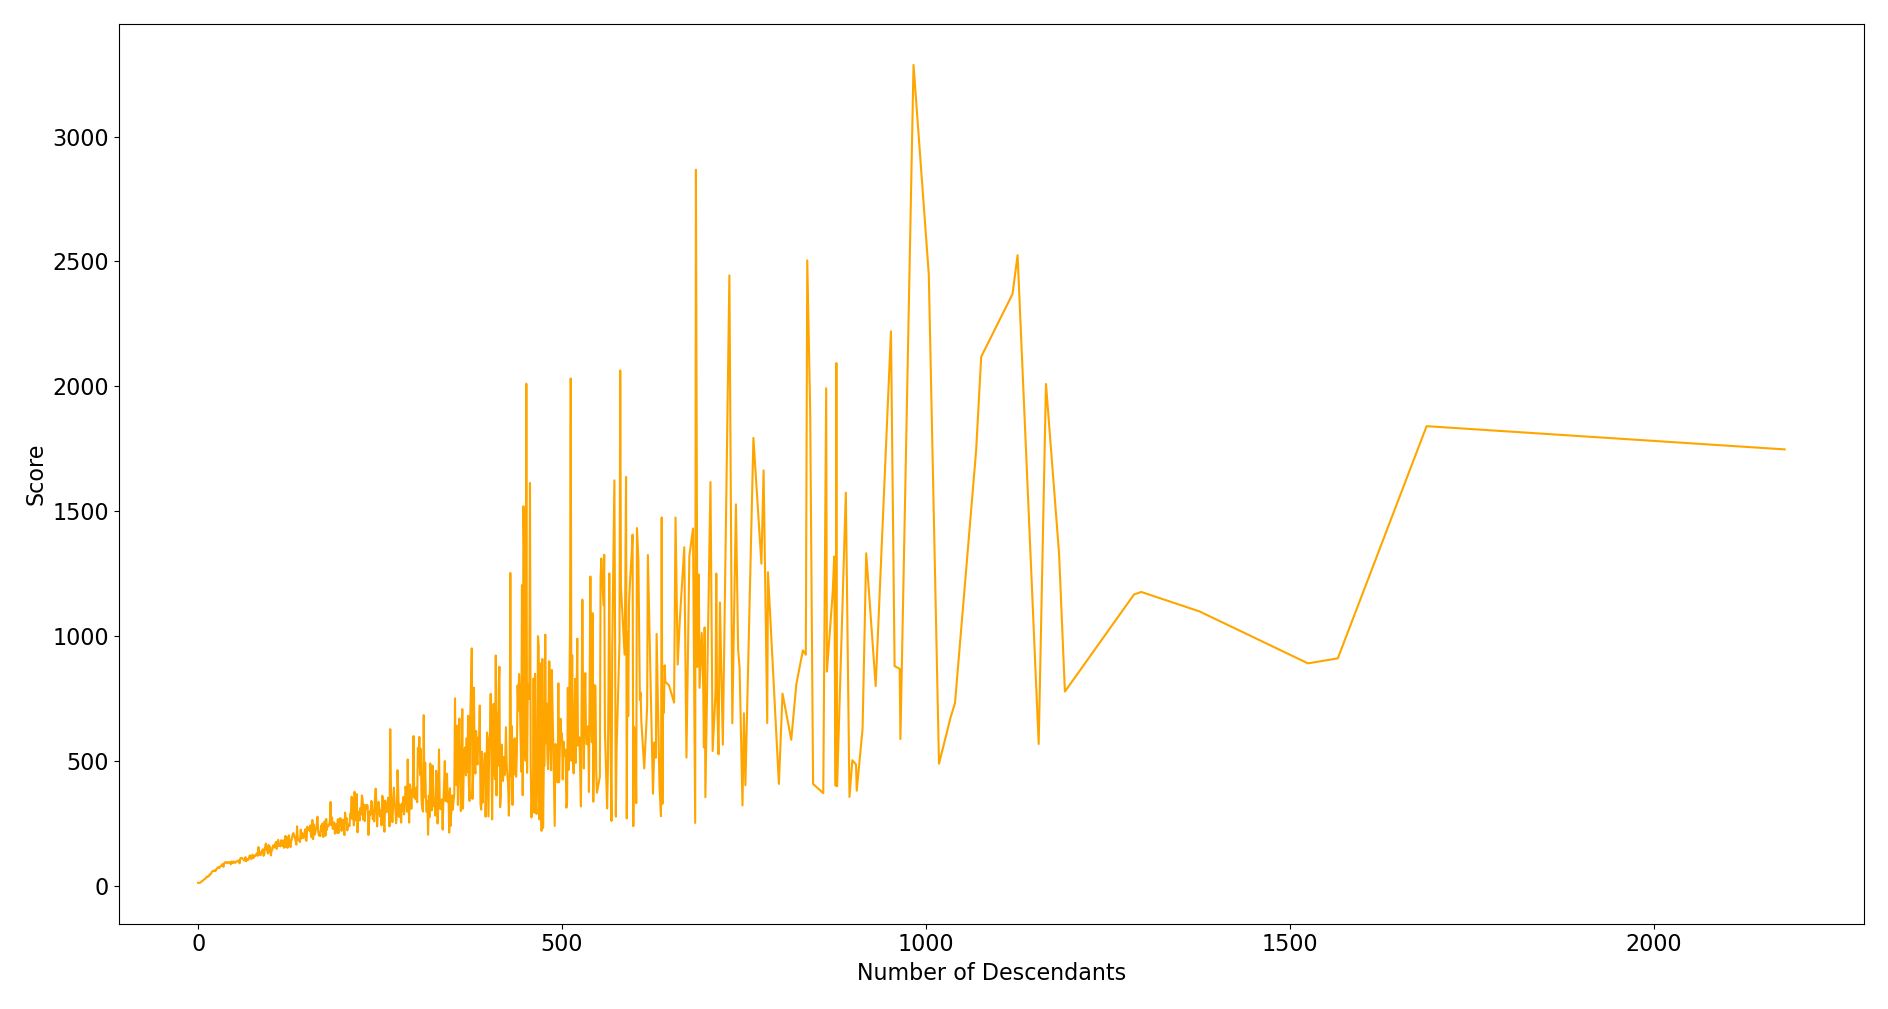
\includegraphics[width=\linewidth]{fig/score_per_descendants.png}
    \caption{Score of story per number of comments}
    \label{fig:heatmap_score_per_dayandhour}
\end{figure}

The average score of a story can be related to the number of comments it
has (user engagement). Usually, a higher number of comments, leads to a
higher score. Up until reaching 500 comments, stories' scores stay below
1000 points. Stories with the highest scores  are found between
the interval of 750 and 1000 number of comments. There isn't enough data
to conclude anything about stories with more than 1000 comments, but the
ones that exist in the dataset, appear to score lower than expected
(about the same as stories with 750 to 1000 comments)
 
\section{Conclusion}
The data analysis allows for the following conclusions: there is enough
data to feed the planned information retrieval system; it is varied in
topics and scopes; the data is of a high quality. All of these factors
and the use of a relational database, to store the data in its final form,
will provide the flexibility and ease of use to advance in the project.\\
With more time, it would be possible to obtain the data relative to all
stories, comments, and possibly even URLs. This would make the temporal
exploration of the data more interesting, allow for the correction of
the approximation made on the comment's descendants count (mentioned in the
\hyperref[sec:post_processing]{Post Processing section}), and create an
even more interesting information retrieval system. Also, it would prove
fruitful to improve the web scrapping part of the pipeline in order to
be able to retrieve textual content from all websites (e.g.: youtube.com)
and some file types (e.g.: PDF, png, jpeg, ...).

\bibliographystyle{ACM-Reference-Format}
\bibliography{sample-bibliography}

\end{document}